\chapter{Część praktyczna - wprowadzenie}
\label{chapter:application}

\newglossaryentry{horizon}{name={Horizon},description={Aplikacje internetowa, do zarządzania chmurzę obliczeniową OpenStack}}

Cześć praktyczna pracy dyplomowej dotyczy implementacji oprogramowania typu \textbf{LaaS} (\ref{chapter:monitoring_architecture:laas}).
W założeniu ma ono stanowić część całego stosu oferowanego przez firmę Fujitsu dla kompleksowego monitorowania chmur obliczeniowych.
Niemniej, możliwe jest również wykorzystanie części lub całości, do monitoringu standardowych systemów informatycznych. 
Specyficzną oraz wyjątkową cechą części praktycznej, oprócz realizowania jej również na płaszczyźnie zawodowej, jest jej otwartość.
Całość implementacji dostępna jest jako oprogramowania otwarte na licencji \textbf{Apache License V2.0}. 
Dzięki temu też, autor poniższej pracy dyplomowej, ma możliwość tworzenia aplikacji we współpracy z takimi firmami:
\begin{itemize}
    \item Hewlett Packard,
    \item Time Warner Cable.
\end{itemize}

Implementacja stanowi rozszerzenie projektu \textbf{monasca}, oryginalnie przygotowanego i opublikowanego przez firmę HP.
W ramach tego rozwiązania można wyróżnić następujące części składowe:
\begin{itemize}
    \item[monasca-api] - REST'owe API, z którym komunikują się pozostałe komponenty, celem zapisywania metryk, alarmów (oraz ich definicji).
    Pozwala także na dostęp do wspomnianych danych.
    \item[monasca-agent] - rozbudowane narzędzie do monitorowania systemu lub aplikacji na maszynie na której został zainstalowany.
    \item[monasca-persister] - prowadzi aktywny nasłuch na kolejce. Wszelkie zmiany stanu na alarmach oraz przekazane metryki, zapisuje,
    poprzez \textbf{monasca-api} do bazy danych.
    \item[monasca-thresh] - jest w stanie, na podstawie zebranych metryk, określić stan w jakim powinien znaleźć się alarm.
    \item[monasca-notification] - na podstawie alarmów, generuje powiadomienie na skonfigurowanego punkty docelowe,
    \item[monasca-ui] - komponent zrealizowany jako wtyczka do \glslink{horizon}{Horizon}, dające wgląd w alarmy, pozwalająca tworzyć ich definicje (monitory).
    Jej główną zaletą jest również wbudowana obsługa do Grafana, która pozwala na przeglądania metryk w czasie rzeczywistym w postaci wykresów.
\end{itemize}
Część praktyczna, jak zostało wcześniej wspomniane, będzie uzupełnieniem dla \textbf{monasca}, praktycznej implementacji
\textbf{MaaS}, o możliwości opisane technologią \textbf{LaaS}.

\section{Architektura aplikacji}
\label{chapter:application:architecture}

\begin{figure}[H]
    \centering
    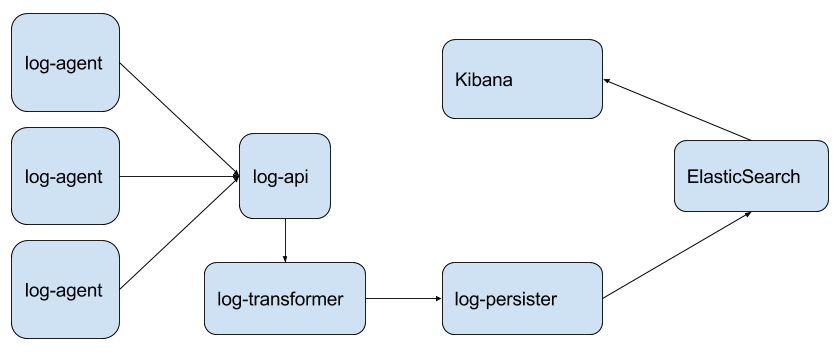
\includegraphics[width=1.0\textwidth]{images/application_arch}
    \caption[Architektura aplikacji]{
        Architektura aplikacji, źródło: opracowanie własne
    }
    \label{chapter:application:architecture:diagram}
\end{figure}

Część praktyczna pracy dyplomowej, przedstawiona na rysunku \ref{chapter:application:architecture:diagram}, 
zaprojektowana została w architekturze rozproszonej - mikro serwisu. Głównym zadaniem takiego rozwiązania
jest rozbicie faktycznej aplikacji na mniejsze programy. Poszczególne części składowe posiadają jedno, 
jasno określone, zadania i jedynie za nie są odpowiedzialne. Niemniej, zasada pojedynczej odpowiedzialności, znana także jako
jeden z wyznaczników dobrej klasy w rozumieniu programowania obiektowego, jest także i tutaj rozumiana w szerszym
kontekście. Pojedynczy serwis współpracuje z innymi. Przykładowa aplikacja mogłaby realizować funkcjonalność 
sklepu internetowego. Jednymi z wielu zamkniętych w środków serwisów, mogłyby by być te odpowiedzialne za zarządzania
klientami lub ogólnie użytkownikami oraz te, których zadaniem byłoby, wsparcie w kierunku zarządzania towarami oferowanymi
przez sklep. Oba, z kolei, wymagałyby wsparcia kolejnego serwisu - bazy danych. Z przedstawionego opisu wynikają jasno pewne
szczególne cechy tego typu architektury:
\begin{itemize}
    \item[\textbf{skalowalność}] - konieczność uruchomienia kolejnych serwisów tego samego typu nie jest trudnym zadaniem. Dzięki temu, 
    że są to aplikacje małe, są one jednocześnie łatwe w zarządzaniu. Ponadto skalowania w kierunku osi OY jest tańsze. Koszt
    dodania średniej mocy maszyny, na której działałaby kolejne instancja serwisu, jest niższy niż dołożenia szybszych podzespołów
    do już istniejącej maszyny, co jest cechą znamienną skalowania wertykalnego,
    \item[\textbf{nauczenie się aplikacji}] - łatwiej jest zrozumieć prostą aplikację, mechanizmy jej działania, aniżeli dogłębnie poznać
    jedną większą. Okazuje się to szczególnie przydatne w dynamicznych zespołach programistów, gdzie rotacja ludzi jest wysoka albo
    częstym zmianą podlegają wymagania,
    \item[\textbf{lepsze izolowanie}] - żaden program nie jest wolny od błędów. Izolowania poszczególnych serwisów jest szczególnie
    przydatne, jeśli dana aplikacja ma problemy z zarządzaniem pamięcią lub przestrzenią dyskową. Inwestygacja mająca 
    na celu ustalenie problemu w dużym programie zajęłaby dużo więcej czasu, nie wspominając już o jego wyeliminowania. 
    W małych aplikacjach ilość wzajemnych korelacji między poszczególnymi jej komponentami jest znacznie niższa od tej
    spotykanych w średnich i dużych programach,
    \item[\textbf{niezależność}] - model aktualizacji lub bardziej ogólnie przekazywania gotowej aplikacji do środowiska produkcyjnego
    staje się również uproszczony. W architekturze mikro-serwisów, każdy serwis może być rozwijany niezależnie od innych i 
    w takiej samej formie, można wypuszczać jego nowe wersje. Jest to także udogodnienie dla klientów, którzy mogą
    pobrać jedynie mały plik binarny lub archiwum. Sam proces aktualizacji jest również narażony na mniejszą ilość
    trudnych do przewidzenia problemu \cite{microservice_architecture}. 
\end{itemize}

Najważniejszą jednak cechą, z którą borykają się systemy informatyczne, jest wyeliminowania \textbf{single-point-of-failure}.
To angielskie pojęcia, w praktyce oznaczana, wadę architektury systemu lub nawet i aplikacji. Najczęściej jednak odnosi się
ona do systemu jako całości. Umieszczenie w jednym miejscu jednej dużej aplikacji lub kilku mniejszych współpracujących 
między sobą, powoduje powstania newralgicznego punktu całego systemu, który jeśli ulegnie awarii, w najlepszy wypadku spowoduje
jedynie opóźnienie w dostarczaniu potrzebnych usług, a w najgorszym całkowicie wyłączy system. Warto w tym miejscu dodać, że
awarie, nie muszą być wcale spowodowane przez sam program. Sytuacje takie jak wyczerpania się pamięci operacyjnej lub 
zajęcia całej mocy obliczeniowej procesora, stanowią ułamek możliwych niefortunnych komplikacji. Należy tutaj brać pod uwagę
także awarię sprzętu, przerwy w dostawie prądu, a także konieczność przeprowadzania prac serwisów lub wymiany istniejących
komponentów komputera na lepsza.  

\subsection{Proces instalacji}
\label{chapter:application:architecture:installation}
    Część praktyczna, jak zostało wcześniej omówione, została zrealizowana w architekturze mikro-serwisów. Warto w tym miejscu dodać,
    że oprócz komponentów omówionych w poniższych rozdziałach, jest to tak naprawdę rozszerzenie istniejącego rozwiązania typu \textbf{MaaS}
    (\ref{chapter:monitoring_architecture:maas}) - monasca. W przypadku tak dużego systemu, składającego się z wielu elementów, 
    konieczne było opracowanie spójnej metody instalacji. Wybór padł na \textbf{Ansible}. 
    
    \subsubsection{Ansible - Simple IT Automation}
    Ansible jest odpowiedzią na pytania - Jak wdrożyć kompleksowy system na więcej niż jednej maszynie. Architektura tego rozwiązania,
    zakłada przygotowanie pakietów instalacyjnych w relacji 1:1 do komponentu, który ma on instalować. Wspomniany pakiet, istnieje pod nazwą roli.
    Jest to najmniejsza cegiełka w całym ekosystemie. Domem, korzystając w dalszej części z metafory, jest tak zwany \textbf{playbook}.
    
    \begin{figure}[H]
        \centering
        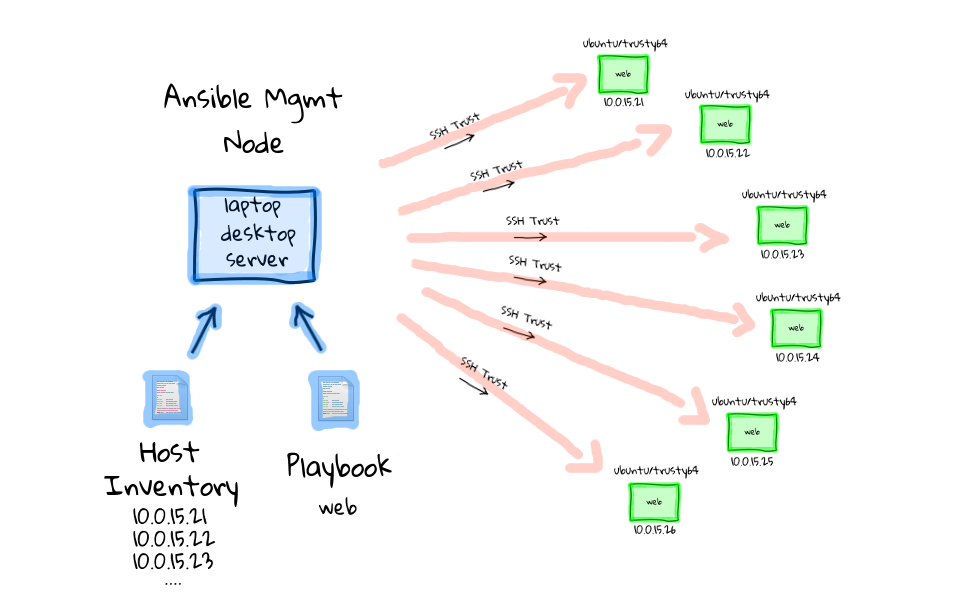
\includegraphics[width=1.0\textwidth]{images/43-ansible-multi-node-deployment-workflow}
        \caption[Wdrożenia z Ansible]{
            Wdrożenia z Ansible, 
            źródło: \url{https://d1cg27r99kkbpq.cloudfront.net/static/extra/43-ansible-multi-node-deployment-workflow.png}
        }
        \label{chapter:application:architecture:installation:ansible_diagram}
    \end{figure}
     
    Pozwala on na budowania scenariusza instalacji według koncepcji przedstawionej na diagramie 
    \ref{chapter:application:architecture:installation:ansible_diagram}. Pojedyncza maszyna, zwana dalej
    maszyną kontrolną, posiada wiedzę o wszystkich hostach wchodzących w skład całego systemu. Na niej
    również zlokalizowane są scenariusze. Ręcznie lub automatyczne zarządzenie infrastrukturą jest
    tutaj aspektem wykraczającym poza ramy pracy dyplomowej, dlatego też nie zostanie omówione. 
    Warto jedynie dodać, że sam proces instalacji na maszynach, możliwy jest do monitorowania na co najmniej
    dwa sposoby:
    
    \begin{itemize}
        \item[Ansible Tower] - rozwiązanie zaprojektowane specjalnie z myślą o monitorowaniu pracy
        procesu wdrożeniowego. Pozwala na przeglądanie listy wszystkich maszyn, obecnego statusu
        zadań (ról),
        \item[Syslog] - wszelka aktywność (tj. operacja), które \textbf{Ansible} wykonuje logowane są
        z użyciem protokołu Syslog na danej maszynie. Dostęp do logów pozwala na prześledzenie operacji oraz
        ewentualnego uzyskania wiedzy na temat przyczyn nieprawidłowego (zakończonego niepowodzeniem) wdrożenia
    \end{itemize}
    
    Najistotniejszą cechą \textbf{Ansible} jest jednak możliwość wskazania, praktycznie nieskończonej,
    ilości maszyn docelowych (fizycznych, wirtualnych lub nawet kontenerów Docker), na których ma zostać ona wprowadzona. 
    Dzięki temu, skalowanie aplikacji na kolejne maszyny, przestaje być operacją problematyczną. Wystarczy dodać 
    informację o jej adresie IP oraz skonfigurować komunikację protokołem SSH.

\section{ELKStack}
\label{chapter:application:elkstack}

\textbf{ELKStack} - akronim opisujący stos technologi składający się z 3 elementów:
\begin{itemize}
    \item[ElasticSearch] - pełnotekstowy silnik wyszukiwania,
    \item[Logstash] - scentralizowane przetwarzania danych,
    \item[Kibana] - interfejs graficzny silnika \textbf{ElasticSearch}
\end{itemize}

\subsection{Logstash}
    Logstash jest wysoce elastycznym narzędziem, nie tylko w kontekście architektury \textbf{ELKStack}.
    Możliwe jest skonfigurowanie go, aby działał jako kolektor danych, jako ich filtr czy też
    transformator. Składa się on z 3 elementów:
    \begin{itemize}
        \item sekcji wejścia,
        \item sekcji przetwarzania,
        \item sekcji wyjścia
    \end{itemize}
    Każda z nich może składać się z więcej niż jednego bloku, opisującego jej zadania.
    Innymi słowy ilość wejść jest nieograniczona tak samo jak możliwości przetworzenia
    odebranych danych oraz ostatecznie wysłania ich do więcej niż jednej lokalizacji.
    Ponadto dla każdej z nich możliwe jest napisania własnego modułu lub wykorzystanie
    jednego z, ciągle rosnącej listy, publicznie dostępnych.
    
    Jest to ponadto rozwiązanie szybkie oraz łatwo skalowalne. Uruchomienie kolejnej
    instancji sprowadza się do przygotowania odpowiedniego pliku konfiguracyjnego
    i dostarczenia go jako argumentu wejściowego do pliku wykonywalnego aplikacji logstash.
    
    \todo[inline]{Opisać korzyści ???}

\subsection{ElasticSearch}
    Pełnotekstowych, indeksowany silnik wyszukiwania. Jednak \textbf{ElasticSearch} jest także
    nierelacyjną bazą danych opartą o koncepcję dokumentów. Możliwość przechowywania oraz wyszukiwania
    informacji pośród zgromadzonych danych, które mogą mieć zarówno ustaloną strukturę, jak i  luźną, jest
    szczególnie istotna dla zarządzania logami. Tym co wyróżnia każdy z nich jest informacja, wiadomość
    zawarta w kolejnych rekordach, a która jest inna dla każdego z nich. 
    
    ElasticSearch oferuje możliwość pełnotekstowej wyszukiwarki na przechowywanych danych, dzięki
    indeksacji. Każda informacja, która wpływa do aplikacji, nie jest po prostu tam zapisywana.
    Specjalnie skonfigurowane indeksy pozwalają na określenie tego, co jest istotne. Ale nie jest
    to konieczne. Jedną z wartych wspomnienia funkcji, jest automatyczna detekcja typów danych, na ich
    podstawie. Wspomniane indeksy są tworzone automatycznie, aby jak najszybciej można było
    wykorzystać możliwości oferowane przez \textbf{ElasticSearch}.
    
    \textbf{Multitenancy}, cecha, wyróżnik chmur obliczeniowych, jest bardzo łatwo do osiągnięcia
    dzięki grupowania i indeksacji w \textbf{ElasticSearch}. Grupa idealnie oddaje koncepcję tenanta.
    Wszystkie dane dla niego zgromadzone mogą zostać odszukane, poprzez wskazania indeksu. Jest on
    tożsamy z grupą, a w dalszej kolejności tenantem.
    
    Jest to także rozwiązania łatwo skalowalne. \textbf{ElasticSearch} posiada ten mechanizm wbudowany.
    Innymi słowy każda nowo uruchomiana instancja poszukuje w sieci, w której działa, innych instancji
    samoistnie budując klaster złożony z lidera oraz replik. 
    Lider odpowiedzialny jest za koordynacją pracy klastra i może również przechowywać dane.
    Repliki stanowią odzwierciedlenie stanu lidera. Jeśli którakolwiek z instancji zostanie wyłączona z klastra,
    potrafi się o samodzielnie przebudować. Dane przesyłane są między replikami. Ostatecznie uzyskuje się
    stan równowagi. Utracenie lidera nie stanowi przeszkody dla poprawnego działania. Pozostałe maszyny 
    negocjują wybór nowego i całość jest ponownie gotowa do świadczenia pełnej funkcjonalności w relatywnie
    krótkim czasie.

    Ostatecznie jest to także \textbf{REST}-owe API. Cała funkcjonalność dostępne jest poprzez
    protokół HTTP. Możliwe jest również administrowaniem klastra przez to samo medium.

\subsection{Kibana}
\label{chapter:application:elkstack:kibana}

    Ostatni z elementów \textbf{ELKStack}. Zadaniem \textbf{Kibana} jest dostarczyć graficznego interfejsu
    użytkownika dla \textbf{ElasticSearch}. Z poziomu aplikacji dostępnej przez przeglądarkę możliwe
    jest przeglądania wszystkich danych zgromadzonych przez \textbf{Logstash} z użyciem tradycyjnych
    metod przeszukiwania:
    \begin{itemize}
        \item filtrowanie,
        \item kwerendy, w tym wypadku pełnotekstowe
    \end{itemize}
    
    Niemniej, to co jest szczególnie użyteczne to wizualizacja danych. Domyślny widok pozwala przeglądać 
    rekordy w formie zbliżonej do tabeli. 
    \begin{figure}[H]
        \centering
        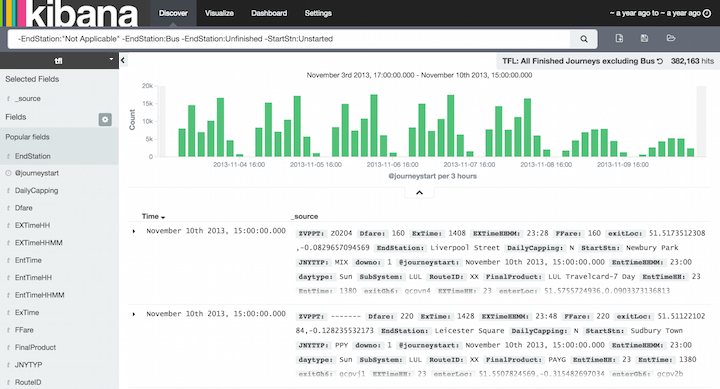
\includegraphics[width=1.0\textwidth]{images/kibana_main_view}
        \caption[Ekran główny w Kibana]{
            Ekran główny w Kibana, źródło: \url{https://www.elastic.co/guide/en/kibana/current/introduction.html}
        }
        \label{chapter:application:elkstack:kibana:main_view}
    \end{figure}
    W tym samym miejscu, można zaobserwować jak Kibana współpracuje z ElasticSearch. Na rysunku \ref{chapter:application:elkstack:kibana:main_view} po lewej stronie widoczny jest pasek szybkiego
    wyszukiwania. Znajdujące się tam pozycje odpowiadają kolejnym właściwościom przeglądanego zbioru danych.
    Korzystając z niego, potencjalny użytkownik, ma możliwość szybkiego filtrowania danych, a ilość filtrów jest
    nieograniczona. Po włączeniu wszystkich szybkiej filtracji, użytkownik w dalszym ciągu, może napisać
    własne zapytania \textbf{QueryDSL} i przesłać je do serwera. Kibana, domyślnie, sortuje dane w kolejności
    rosnącej względem skonfigurowanego pola dla danego indeksu. Rekordy można oglądać w dowolnym wycinku czasu.
    
    Szczególnie interesującą cechą wyników wyszukiwań, które można przeglądać w Kibana, jest to, że bezboleśnie
    łączą się one z dowolną formą wizualizacji. I tak samo, jak użytkownik, mógłby chcieć przejrzeć dane 
    jedynie z konkretnych dwóch godzin, konkretnego dnia, tak samo, możliwe jest uruchomienie podobnego
    filtru dla wykresu kołowego lub słupkowego.
    \begin{figure}[H]
        \centering
        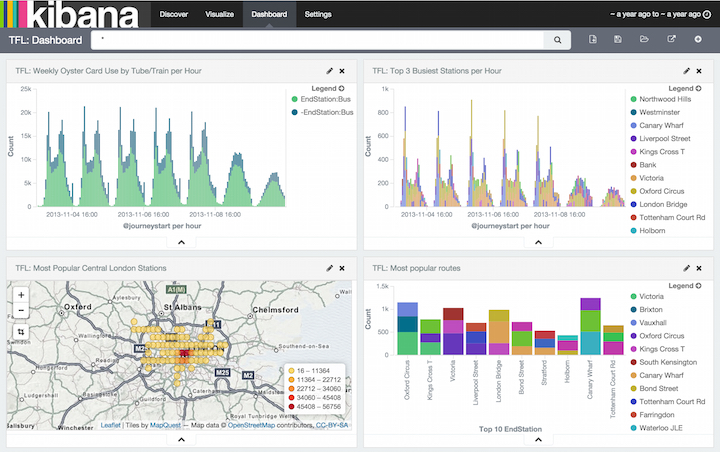
\includegraphics[width=1.0\textwidth]{images/kibana_dashboards}
        \caption[Ekran współdzielony w Kibana]{
            Ekran współdzielony w Kibana, źródło: \url{https://www.elastic.co/guide/en/kibana/current/introduction.html}
        }
        \label{chapter:application:elkstack:kibana:dashboard}
    \end{figure}
    Wykresy, w dalszym ciągu można łączyć w tak zwane \textbf{dashboards}, które stanowią idealne narzędzia do kolaboracji
    w tym samym zespole. Prócz tego, że pozwalają ona na pokazanie jednocześnie więcej niż jednej wizualizacji, z których
    każda odnosi się do samego momentu w czasie, da się je zapisywać i przekazywać innym członkom zespołu. 
\section{monasca-log-agent - zbieranie logów}
\label{chapter:monasca:monasca_log_agent}

    \subsection{Znaczenie komponentu}
    \textbf{monasca-log-agent} jest praktyczną implementacją koncepcji monitorowania aplikacji opartej o agentów.
    Agent zlokalizowany jest więc najbliżej danych, które ma zbierać, a które ma za zadanie przetworzyć i wyniki
    przesłać dalej. Jest to efektywne podejście z uwagi na wolumin danych. Tempo oraz ilość generowanych logów
    może być znacząca, dlatego też pobieranie danych poprzez sieć, znacząco wydłużałoby całkowity czas 
    wszystkich operacji, jakie agent musi wykonać.
    
    \todo[inline]{schemat rozmieszczania agentów, linie schodzą się do monasca-log-api}
    
    Agent został oparty o jeden z elementów stosu technologicznego \textbf{ELKStack} - \textbf{Logstash}.
    Do zadań agenta należy:
    \begin{itemize}
        \item obserwacja wskazanego pliku z logami,
        \item wykrywania i łączenie wpisów składających się z wielu linii,
        \item dodawania informacji o tenancie chmury obliczeniowej,
        \item wskazywania na typ aplikacji, z której logi są zbierane,
        \item wysyłania danych do \textbf{monasca-log-api} \ref{chapter:monasca:monasca_log_api}
    \end{itemize}
    
    Konfiguracja agenta odbywa się w sposób deklaratywny, poprzez plik konfiguracyjny. Poprawne
    skonfigurowanie sprowadza się do:
    \begin{itemize}
        \item wskazania źródła danych,
        \item określenia miejsca docelowego, do którego dane mają zostać wysłane
    \end{itemize}
    W przypadku monitorowania logów, konfiguracja jest bardziej rozbudowane.
    Agent musi zwrócić szczególną uwagę na problem wpisów, które znajdują się w więcej niż jednej linii.
    Najczęściej ten problem objawia się, gdy aplikacja zgłasza błędy, a logach pojawią się rekordy, które
    te problemy opisują. Do opisu błędu (w kontekście logowania) dodawany jest tak zwany \textbf{stacktrace}.
    Zawiera on szczegółowy zrzut wywołań kolejnych funkcji, w różnych modułach, w wyniku których aplikacja
    nie wykonała poprawnie danego zadania. \textbf{Stacktrace}, dla łatwości odczytu przez człowieka,
    jest najczęściej reprezentowany w postaci wpisu zajmującego wiele linii. Z punktu widzenia domyślnej
    konfiguracji \textbf{logstash} kolejne linii to zupełnie odrębne wydarzenia. Dla administratora systemu jest
    to jednak logicznie spójna całość, którą on sam analizował by w takim kontekście. Agent musi więc wiedzieć,
    w jaki sposób połączyć oddzielnie linie w jedno i w takiej formie przesłać je do wyjścia.
    
    \subsection{Problem wielu linii}
    
    \subsection{Konfiguracja agenta}
        \todo[inline]{przykładowa konfiguracja}
        
        \subsubsection{Obserwacja wskazanego pliku z logami}
            Do konfiguracji logstash'a przekazywana jest ścieżka lub wyrażenia regularnego wskazującego
            na, odpowiednio, plik lub listę plików, z których odczytywana mają być rekordy. \textbf{Logstash}
            wykonuje to zadanie podobnie do Linuksowego narzędzia \textbf{tail}. Kolejne zdarzenia w danej 
            instancji agenta, to kolejne linii w obserwowanych plikach, pojawiające się na ich końcu. 
        
        \subsubsection{Wykrywania i łączenie wpisów składających się z wielu linii}
            Problem ten rozwiązany jest z użyciem następującego algorytmu:
            \begin{enumerate}
                \item określenie jaki typ aplikacji jest monitorowany,
                \item utworzenia adekwatnego wyrażenia regularnego opisującego początek lub koniec wydarzenia,
                \item określenie kierunku łączenia kolejnych rekordów
            \end{enumerate}
            \todo[inline]{Ansible i przygotowane szablony dla multiline}
            
        \subsubsection{Dodawania informacji o tenancie chmury obliczeniowej}
            Agent, jak zostało to wcześniej wspomniane, działa na konkretnej maszynie. Jedną z jej własności jest
            informacja o użytkowniku - tenancie - unikatowy numer UUID. W przypadku logowania jako serwisu,
            szczególnie istotna jest wiedza właśnie o użytkowniku chmury, na rzecz którego, dane logi zostały
            zebrane. \textbf{monasca-log-agent} rozwiązuje ten problem z wykorzystaniem biblioteki \textbf{keystone}
            \footnote{Keystone - aplikacja mająca za zadania rozwiązać problem autentykacji oraz autoryzacji w
                chmurach obliczeniowych Openstack}. 
            Agent, tuż przed przesłanie logu do \textbf{monasca-log-api} wykonuje procedurę logowania do chmury
            używając, dostarczonych w konfiguracji, nazwy użytkownika oraz hasła. Jako wynik, jeśli logowanie 
            zakończyło się sukcesem, otrzymuje token oraz numer tenanta. Dołączony jest on do logu.
            
        \subsubsection{Wskazania na aplikację}
            Informacja o logu zostaje wzbogacona o dane, które pozwalają określić typ oraz samą aplikacją.
            
         \subsubsection{Wysyłanie danych do monasca-log-api}
             Wysyłania danych do monasca-log-api jest poprzedzone logowanie do chmury obliczeniowej, jeśli nie
             zostało ono wcześniej wykonane lub jeśli token wygasł. Po udanej autentykacji, kolejne rekordy
             z logu przesyłane są pojedynczo do serwera, gdzie działa \textbf{monasca-log-api}.
\section{monasca-log-api - REST'owe API dla logów}
\label{chapter:monasca:monasca_log_api}

\textbf{monasca-log-api} jest to \textbf{REST}-owe API skonstruowane jako
brama wejściowa do odbierania logów od agentów (instancje \textbf{monasca-log-agent}
\ref{chapter:monasca:monasca_log_agent}).
    
    \subsection{Proces przysyłania danych}
    \begin{figure}[H]
        \centering
        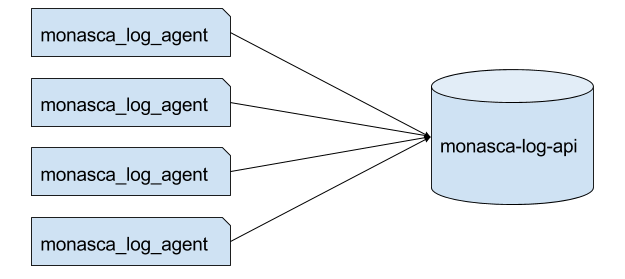
\includegraphics[width=0.80\textwidth]{images/monasca_log_api_data_flow}
        \caption[Relacja monasca-log-agent z monasca-log-api]{
            Relacja monasca-log-agent z monasca-log-api, źródło: opracowanie własne
        }
        \label{chapter:monasca:monasca_log_api:data_flow}
    \end{figure}
    Przesył danych inicjowany jest po stronie agenta. To, co zostanie przesłane
    do \textbf{monasca-log-api}, zależy w dużej mierze od konfiguracji agenta 
    \ref{chapter:monasca:monasca_log_agent:configuration}. Oprócz faktycznego
    logu, agent dodaje najczęściej informacje pozwalające na ustalenie jego pochodzenia (ścieżki, aplikacji) oraz
    datę pobrania rekordu. Po skompletowaniu wszystkich informacji wiadomość podlega
    transformacji do żądania HTTP i zostaje wysłana do serwera.
    
    \subsubsection{Struktura żądania}
    \begin{figure}[h]
        \centering
        
\includegraphics[width=0.80\textwidth]{images/monasca_log_api_request}
        \caption[Żądanie HTTP w monasca-log-api]{
             Żądanie HTTP w monasca-log-api, źródło: opracowanie własne
        }
        \label{chapter:monasca:monasca_log_api:request}
    \end{figure}
    Rysunek \ref{chapter:monasca:monasca_log_api:request} przedstawia przykładowe
    żądanie, jakie agent może wysłać do serwera, w postaci minimalnie wymaganej
    i akceptowanej przez aplikację. Nagłówki żądania:
    \begin{itemize}
        \item \textbf{X-Tenant-Id} - UUID jednoznacznie identyfikujący tenanta w chmurze,
        \item \textbf{X-Application-Type} - wskazuje na typ aplikacji, z której zebrano logi,
        \item \textbf{X-Dimensions} - wszelkie dane opisujące żądanie (nazwa hosta, adres IP hosta itp) 
    \end{itemize}
    stanowią rodzaj uzupełniania dla logu, przesłanego w ciele żądania. Faktyczna ilość nagłówków wygląda 
    jednak inaczej. W wyniku weryfikacji wartości \textbf{X-Tenant-Id}, do listy dołączane są:
    \begin{itemize}
        \item \textbf{X-Identity-Status} - określający status autentykacji,
        \item \textbf{X-Roles} - zestaw uprawnień powiązanych z tenantem.
    \end{itemize}
    
    Również ciało żądania może być dużo większe. Niemniej jest to najczęściej łańcuch tekstowy
    interpretowany jako \textbf{application/json}, który zawierać będzie przynajmniej pole \textbf{message},
    ostatni odczytany wpis w monitorowanego pliku. Na rozmiar żądania natomiast, największy wpływ będzie mieć
    to jak duży był log (na poziomie obserwowanego zasobu). 
    
    Każdy z agentów wysyła kolejne rekordy z monitorowanych plików pojedynczo jako
    ciało żądania HTTP\footnote{Request body lub message body - dane, które klient wysyła do serwera}.
    Zawiera ono surowe dane odczytane przez agenta. \textbf{monasca-log-api} nie zajmuje się normalizacją lub weryfikacją tych danych. Głównym tego powodem jest fakt, że struktura logu na poziomie
    serwera WWW jest rzeczą nieznaną. Wynika to z ilości potencjalnych źródeł, które 
    mogą przesyłać do niego dane. Niemniej walidacja istnieje, ale odnosi się do:
    \begin{itemize}
        \item rozmiaru przesłanych danych (walidacja dwupoziomowa),
        \item nagłówków żądania, które muszę odpowiadać ustalonemu formatowi
    \end{itemize}\cite{monasca_log_api_spec}.
    
    \subsubsection{Proces walidacji}
    \label{chapter:monasca:monasca_log_api:validation}
    
    Serwer nie przetworzy każdego żądania. Jednym z kryterium odrzucenia i
    tym samym walidacji jest rozmiar przesłanych danych. Konieczność wykonania tego kroku, 
    związana jest z elementem odbierającym dane od \textbf{monasca-log-api}, a dokładniej z medium
    którymi informacje są przesyłane. \textbf{Kafka} - kolejka danych - może, w domyślnej konfiguracji,
    przyjąć jednorazowo 1MB (megabajt) danych. \textbf{monasca-log-api} pro-aktywnie eliminuje zbyt duże
    wiadomości, których próba wysłania zakończyłaby się niepowodzeniem. Walidacja odbywa się na dwóch poziomach.
    \begin{itemize}
        \item[Poziom 0] - weryfikowany jest rozmiar samego żądania HTTP. Pod uwagę brany jest nagłówek
        \textbf{Content-Length}, dający informację o ilości (w bajtach) wysłanych przez klienta danych.
        Przekroczenie maksymalnej wartości powoduje wygenerowanie, przez serwer, odpowiedzi 
        \textbf{HTTP 413 :: Request Entity Too Large}. Wspomniany nagłówek jest szczególnie istotny,
        ponieważ pozwala na określenie, czy żądanie można lub nie przetworzyć, bez konieczności
        odczytania właściwych danych. Z tego też powodu, jego brak, również uznawany jest za błąd.
        W odpowiedzi do klienta serwer wygeneruje błąd \textbf{HTTP 411 - Length Required}.
        \item[Poziom 1] - następuje tuż przed wysłaniem wiadomości do \textbf{Kafki}. Po wykonaniu wszystkich
        operacji, związanych z odczytem żądania, dodaniem meta danych do logu, rozmiar wiadomości może się
        znacząco zwiększyć. Możliwa jest sytuacja, w której początkowy rozmiar jest zbliżony do 
        wartości maksymalnej, ale jej nie przekracza. \textbf{monasca-log-api} nie reaguje na poziomie 0. Wiadomość wysyłana do \textbf{Kafki} składa się jednak z większej ilości elementów,
        więc dodawanie ich może spowodować przekroczenie wartości granicznej. W tym wypadku jest to sytuacja
        tożsama z wewnętrznym błędem serwera, w jej wyniku, klient otrzyma odpowiedź
        \textbf{HTTP 500 - Internal Server Error}.
    \end{itemize}
    
    Warto w tym miejscu zaznaczyć, że zmiany w konfiguracji Kafki, odnoszące się do zwiększania
    maksymalnego rozmiaru wiadomości, są również odzwierciedlane w \textbf{monasca-log-api}. 
    
    \subsection{Dostarczanie danych}
    \begin{figure}[H]
        \centering
        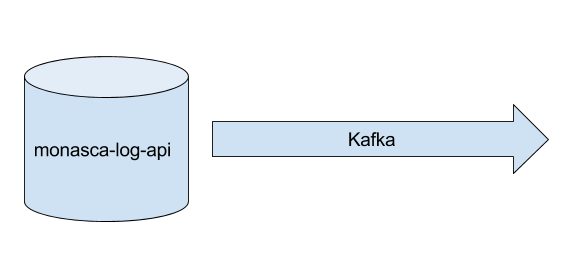
\includegraphics[width=0.80\textwidth]{images/monasca_log_api_to_kafka}
        \caption[monasca-log-api a Kafka]{
            monasca-log-api a Kafka, źródło: opracowanie własne
        }
        \label{chapter:monasca:monasca_log_api:kafka}
    \end{figure}
    Dane z \textbf{monasca-log-api} trafiają do kolejki \textbf{Kafka}.
    Dla każdej z wiadomości obliczana jest specjalna wartość - klucz. Pozwala on na określenia partycji
    wewnątrz Kafki. Dzięki temu dane dystrybuowane są równomiernie. Jest to konieczne z uwagi
    na wolumin danych, które muszą wejść do kolejki. Bez tej operacji mogłoby dojść do przepełnienia się
    bufora wewnątrz Kafki i wiadomości mogłyby zostać utracone. W przypadku logów, o strategicznym
    znaczeniu dla chociażby analizowania przyczyn potencjalnych błędów, jest to sytuacja niedopuszczalna.
    
\section{monasca-log-transformer - proste transformacje}
\label{chapter:monasca:monasca_log_transformer}

\textbf{monasca-log-transformer} jest komponentem znajdującym się bezpośrednio
za \textbf{monasca-log-api}. Jest to ponownie specjalnie skonfigurowana instancje
\textbf{Logstash} \ref{chapter:application:elkstack}. Nasłuchuje on na \textbf{topic}'ach w oczekiwaniu
na wiadomości, które \textbf{monasca-log-api} na nie wysyła. 
\newglossaryentry{kafka_topic}{
    name={Topic},
    description={Topic jest w Kafce tożsamy z grupą. Podczas gdy jedna aplikacja wpisuje dane do wskazanej grupy, inne mogą czytać wiadomości zaadresowane
        do tej grupy. Możliwe jest również czytanie z większej ilości grup}
    }

Po odebraniu wiadomości transformer ma zadanie dokonać, zgodnie z nazwą transformacji, otrzymanego 
logu. Na obecną chwilę jedyną operacją, którą ma za zadanie wykonać jest analiza rekordu pobranego z logu,
aby wykryć jego poziom. Implementacja opiera się na wyrażeniu regularnym, którym objęty jest wycinek
całego logu. W wyniku działania wyrażenia regularnego, do struktury całej wiadomości dodawana jest informacja
o poziomie logu. 

\begin{listing}
    \inputminted[
    fontfamily=monospace,
    fontsize=\scriptsize,
    obeytabs=true,
    samepage=true
    ]{rb}{listingings/transformer.conf}
    \caption[Przykładowa konfiguracja monasca-log-transformer]{
        Przykładowa konfiguracja monasca-log-transformer, źródło: \url{https://raw.githubusercontent.com/FujitsuEnablingSoftwareTechnologyGmbH/ansible-monasca-elkstack/master/templates/transformer.conf.j2}}
    \label{chapter:monasca:monasca_log_transformer:configuration_code}
\end{listing}

Powyższy (\ref{chapter:monasca:monasca_log_transformer:configuration_code}) wycinek kodu przedstawia
sekcję filtracji programu Logstash. Zawarty w niej kod Ruby oraz dopasowanie Grok pozwala na 
pobranie poziomu logu oraz znormalizowania jej do spójnej wartości. 
\section{monasca-log-persister - zapisanie logów do bazy danych}
\label{chapter:monasca:monasca_log_persister}

\textbf{monasca-log-persister} jest ostatnim etapem przed umieszczeniem logów w bazie danych \textbf{ElasticSearch}.
Implementacja została oparta o program \textbf{Logstash}. Prócz zapisu danych do miejsca docelowego, zadaniem
aplikacji jest uzupełnienie logów do postaci, która będzie zrozumiała dla \textbf{ElasticSearch}. 

\begin{listing}
    \inputminted[
    fontfamily=monospace,
    fontsize=\scriptsize,
    obeytabs=true,
    samepage=true
    ]{json}{listingings/persister_input_event.json}
    \label{chapter:monasca:monasca_log_persister:input_message}
    \caption[Przykładowe dane wejściowe dla monasca-log-persister]{
        Przykładowe dane wejściowe dla monasca-log-persister, źródło: opracowanie własne}
\end{listing}

Temu procesowi poddawane są pola takie jak:
\begin{itemize}
    \item[timestamp] - domyślne pole \textbf{@timestamp} generowane jest dla zdarzenia przez \textbf{Logstash}. W przypadku
    logu ważne jest aby ten czas oraz czas, w którym rekord został wygenerowany były tożsame. Dlatego też, program, jeśli
    odnajdzie takową informację w strukturze opisującą log, używa jej jako czasu utworzenia struktury wydarzenia przez instancję
    \textbf{monasca-log-persister}. Dzięki temu, to moment wygenerowania rekordu, jest realnym czasem, według której, w dalszej
    kolejności kolejne pozycje będą sortowane w Kibana.
    \item[creation-time] - znacznik czasowy, wskazujący na odebrania i przetworzenia rekordu przez \textbf{monasca-log-api}.
    \item[dimensions] - \textbf{monasca-log-persister} przenosi wszystkie wartości ustawione w tym polu, do poziomu struktury
    jaką jest zdarzenie.
    \item[application-type] - pole wskazujące na aplikację, która wygenerowała log, podobnie jak \textit{dimensions}, jest przenoszone
    do samego wydarzenia
\end{itemize}

Podobnej operacji podlegają także następujące pola, które oryginalnie zawarte są w logu:
\begin{itemize}
    \item[message] - oryginalna wiadomość, która została pobrana przez \textbf{monasca-log-agent},
    \item[level] - poziom logu przenoszony jest do poziomu wydarzenia jako \textbf{log\_level},
    \item[tenant\_id] - identyfikator użytkownika,
    \item[region] - informacja o regionie, w którym znajdowała się maszyna, a z której pochodzi log,
    \item[path] - ścieżka do pliku, z której pochodzą dane
\end{itemize}